\actTitle{4.1 - Angles and Their Measure}

\videoLink{Section 4.1}{https://www.youtube.com/playlist?list=PLYHZK3b8UFw3HtpDsf1SA0Znm5\_7bAGBY}

\noindent \textbf{Topics:}  angles, degrees, radians, coterminal angles lengths of circular arcs, areas of circular sectors\\

\noindent \textbf{Student Learning Outcomes:}
\begin{enumerate}
\item Students will be able to find degree and radian measure.
\item Students will be able to determine coterminal angles.
\item Students will be able to determine arc length and area of a sector of a circle.
\end{enumerate}

\hrule 

\bigskip

\subsection{Finding Degree Measure} ~

\begin{tabular}{| l |}\hline 
$\star$ An \textbf{angle} is formed by rotating a ray around its endpoint.\\
$\star$  The original position of the ray is called the \textbf{initial side} of the angle;\\ the ending position of the ray is called the \textbf{terminal side}.\\
$\star$  The endpoint of the ray is called the \textbf{vertex}.\\
\hline
\end{tabular}

     \begin{tikzpicture}[y=3.0cm, x=3.0cm,font=\sffamily]
        \begin{scope} %[shift={(0,8)}]
          \draw[thick,<->]
                (1,0) --  (0,0) node[anchor=north,pos=0.5,font=\scriptsize] {Initial Side}
                -- (45:1) node[anchor=east,pos=0,font=\scriptsize] {Vertex}
                          node[anchor=south east,pos=0.5,font=\scriptsize] {Terminal Side}; 
          \fill[black] (0,0) circle [radius=0.4ex];
          \end{scope}
        \begin{scope}[shift={(-1.5,-1)},scale=0.75]
          \draw[thick,<->] (1,0) -- (0,0) -- (-1,0) ; 
          \fill[black] (0,0) circle [radius=0.4ex] node[anchor=south,font=\scriptsize] {Straight angle};
          \end{scope}
        \begin{scope}[shift={(0,-1)},scale=1.0]
          \draw[thick,<->] (1,0) -- (0,0) -- (45:1);
          \draw[thin,black,->] (0.5,0) arc (0:42:0.5);
          \fill[black] (0,0) circle [radius=0.4ex] node[anchor=north west,font=\scriptsize] {Positive angle};
          \end{scope}
        \begin{scope}[shift={(1.5,-0.3)},scale=1.0]
          \draw[thick,<->] (1,0) -- (0,0) -- (-45:1);
          \draw[thin,black,->] (0.5,0) arc (0:-42:0.5);
          \fill[black] (0,0) circle [radius=0.4ex] node[anchor=south west,font=\scriptsize] {Negative angle};
          \end{scope}
        \end{tikzpicture}



\noindent \begin{tabular}{| l | }
\hline $\star$ An angle is said to be in \textbf{standard position} if its vertex is at the origin and its initial side is on the\\ positive $x$-axis.  \\
$\star$ An angle is \textbf{positive} if it is rotated counterclockwise and \textbf{negative} if it is rotated clockwise.\\
$\star$ Greek letters are commonly used to name the angles: $\alpha$ (alpha), $\beta$ (beta), $\theta$ (theta), $\gamma$ (gamma), $\phi$ (phi).  \\ \hline
\end{tabular}






\begin{enumerate}
\item Draw a positive angle $\theta$ in standard position with its terminal side in Quadrant 3 and a negative angle $\beta$ with its terminal side in Quadrant 4.\\[1in]

\newpage
\textbf{Degree Measure}  We can measure angles using degrees noted by $^\circ$.\\[1.3in]
Certain angles have special names:

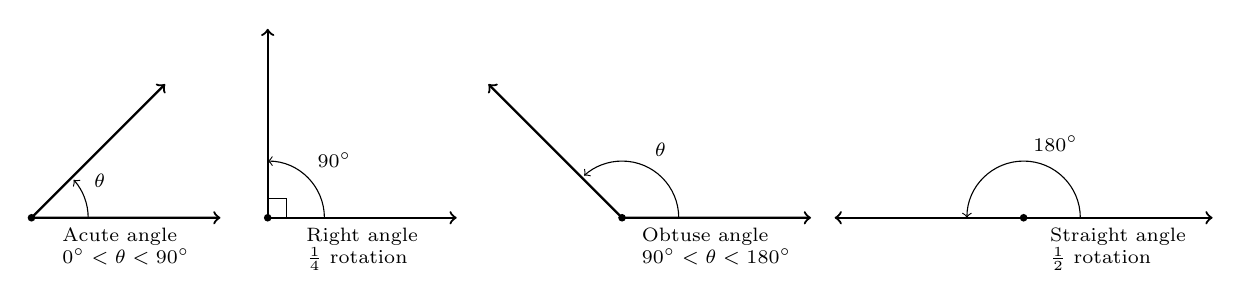
\begin{tikzpicture}[y=3.0cm, x=3.0cm,font=\sffamily]
    \begin{scope}[shift={(0,0)},scale=0.8]
          \draw[thick,<->] (1,0) -- (0,0)
               node[anchor=north,font=\scriptsize,align=left,pos=0.5] {Acute angle\\$0^\circ<\theta<90^\circ$}
              -- (45:1);
          \draw[thin,black,->] (0.3,0) arc (0:42:0.3)
              node[anchor=south west,font=\scriptsize,pos=0.5] {$\theta$};
          \fill[black] (0,0) circle [radius=0.4ex];
    \end{scope}
    \begin{scope}[shift={(1,0)},scale=0.8]
          \draw[thick,<->] (1,0) -- (0,0)
               node[anchor=north,font=\scriptsize,align=left,pos=0.5] {Right angle \\ $\frac{1}{4}$ rotation}
               -- (90:1);
          \draw[thin] (0.1,0) -- (0.1,0.1) -- (0,0.1);
          \draw[thin,black,->] (0.3,0) arc (0:90:0.3)
              node[anchor=south west,font=\scriptsize,pos=0.5] {$90^\circ$};
          \fill[black] (0,0) circle [radius=0.4ex];
    \end{scope}
    \begin{scope}[shift={(2.5,0)},scale=0.8]
          \draw[thick,<->] (1,0) -- (0,0)
               node[anchor=north,font=\scriptsize,align=left,pos=0.5] {Obtuse angle\\$90^\circ<\theta<180^\circ$}
              -- (135:1);
          \draw[thin,black,->] (0.3,0) arc (0:132:0.3)
              node[anchor=south west,font=\scriptsize,pos=0.5] {$\theta$};
          \fill[black] (0,0) circle [radius=0.4ex];
    \end{scope}
    \begin{scope}[shift={(4.2,0)},scale=0.8]
          \draw[thick,<->] (1,0) -- (0,0)
               node[anchor=north,font=\scriptsize,align=left,pos=0.5] {Straight angle \\ $\frac{1}{2}$ rotation}
              -- (180:1);
          \draw[thin,black,->] (0.3,0) arc (0:180:0.3)
              node[anchor=south west,font=\scriptsize,pos=0.5] {$180^\circ$};
          \fill[black] (0,0) circle [radius=0.4ex];
    \end{scope}
\end{tikzpicture}


How many degrees does it take to make a full circle?



\subsection{Finding Radian Measure} ~

\textbf{Radian Measure} To define radian measure we will use a circle
of radius $r$ and the central angle $\theta$.  $\theta$ has a measure
of \textbf{one radian} if it intercepts an arc of length equal to the
radius of the circle.

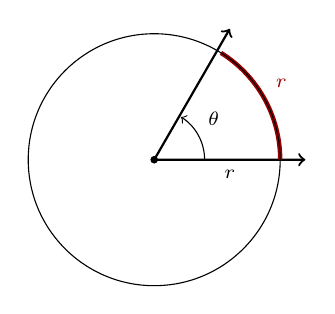
\begin{tikzpicture}[y=2cm, x=2cm,font=\sffamily]
    \begin{scope}[shift={(0,0)},scale=0.8]
          \draw[thick,<->] (1.2,0) -- (0,0)
               node[anchor=north,font=\scriptsize,align=left,pos=0.5] {$r$}
              -- (60:1.2);
          \draw[thin,black,->] (0.4,0) arc (0:58:0.4)
              node[anchor=south west,font=\scriptsize,pos=0.5] {$\theta$};
          \draw[ultra thick,red!60!black] (1,0) arc (0:58:1)
              node[anchor=south west,font=\scriptsize,pos=0.5] {$r$};
          \draw[black] (0,0) circle(1);
          \fill[black] (0,0) circle [radius=0.4ex];
    \end{scope}
\end{tikzpicture}


\item If a circle has a radius of 5 and $\theta$ intercepts an arc of
  length 10, what is $\theta$?
  \vfill

\hspace{-.35in}
\begin{tabular}{ | l | } \hline
  The \emph{radian} measurement of an angle is the number of radii that can be laid out on the \\
  subtended arc. In other words, $\theta = \dfrac{\text{arc length}\, s}{\text{radius}\, r}$. \\
  \\ \hline
\end{tabular}
\newpage

\item How do we convert degrees to radians and radians to degrees?\\
\textbf{Answer:}  We use the complete rotation of a circle.
\begin{center}
1 rotation=$360^\circ$, Circumference of a circle=$2\pi r$
\end{center}
$$\theta=\frac{s}{r}=\frac{\text{circumference}}{r}=\frac{2\pi r}{r}=2\pi$$
Therefore, 1 rotation is $360^\circ=2\pi$ radians.\\
What if we divide both sides by 2?\\[.2in]

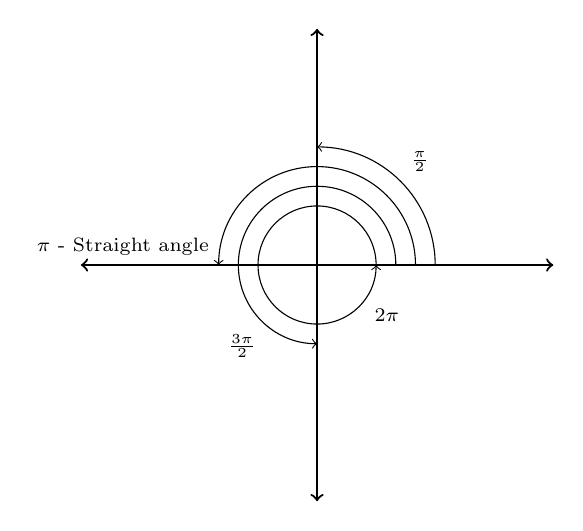
\begin{tikzpicture}[y=2.5cm, x=2.5cm,font=\sffamily]
    \begin{scope}[shift={(0,0)},scale=1.0]
          \draw[thick,<->] (-1.2,0) -- (1.2,0);
               %node[anchor=north east,font=\scriptsize,align=left,pos=0.0] {straight angle};
          \draw[thick,<->] (0,-1.2) -- (0,1.2);
          \draw[thin,black,->] (0.6,0) arc (0:90:0.6)
              node[anchor=south west,font=\scriptsize,pos=0.5] {$\frac{\pi}{2}$};
          \draw[thin,black,->] (0.5,0) arc (0:180:0.5)
              node[anchor=south east,font=\scriptsize,pos=1] {$\pi$ - Straight angle};
          \draw[thin,black,->] (0.4,0) arc (0:270:0.4)
              node[anchor=north east,font=\scriptsize,pos=0.85] {$\frac{3\pi}{2}$};
          \draw[thin,black,->] (0.3,0) arc (0:360:0.3)
              node[anchor=north west,font=\scriptsize,pos=0.9] {$2\pi$};
    \end{scope}
\end{tikzpicture}


\textbf{Conversions}\\
To covert from degrees to radians, multiply by $\frac{\pi}{180}$.\\[.2in]
To covert from radians to degrees, multiply by $\frac{180}{\pi}$.\\

\item Covert $90^\circ, 150^\circ, 1^\circ, -135^\circ$ to radians.\\[1in]
\newpage

\item Covert $\frac{5\pi}{6}, \frac{-5\pi}{6}, 3\pi, 1$ radian to degrees.\\[1in]



\subsection{Coterminal Angles} ~

\textbf{Coterminal Angles} Two angles are coterminal angles if they
have the same terminal side and initial side but different rotations.

\begin{tikzpicture}[y=3.5cm, x=3.5cm,font=\sffamily]
    \begin{scope}[shift={(0,0)},scale=1.0]
          \draw[thick,<->] (-1.0,0) -- (1.2,0)
             node[anchor=north,font=\scriptsize,align=left,pos=0.8] {Initial Side}
             node[anchor=north,font=\scriptsize,align=left] {$x$};
          \draw[thick,<->] (0,-1) -- (0,1)
              node[anchor=east,font=\scriptsize,align=left] {$y$};
          \draw[thick,->] (0,0) -- (30:1)
              node[anchor=east,font=\scriptsize,align=left] {$y$}
              node[anchor=south west,font=\scriptsize] {Terminal Side};
          \draw[thin,black,->] (0.4,0) arc (0:30:0.4)
              node[anchor=south west,font=\scriptsize,pos=0.5] {$30^\circ$};
          \draw[thin,black,->] (0.3,0) arc (0:390:0.3)
              node[anchor=north west,font=\scriptsize,pos=0.75] {$390^\circ$};
    \end{scope}
\end{tikzpicture}



\item Find two positive angles and two negative angles coterminal to $\theta = 60^\circ$.  \\[1in]

\subsection{Arc Length and Area of a Sector} ~


\begin{tabular}{| l |}\hline
If $\theta$ is the radian measure of a central angle of a circle of radius $r$, and if $A$ is the area of \\the circular sector determined by $\theta$, then $A = \frac{1}{2}r^2 \theta$.  \\ \hline
\end{tabular} 
\vspace{-.1in}
\item Determine the area of the circular sector with central angle $\theta = 120^\circ$ when the radius of the circle is 5. \\[.7in]



\item \begin{enumerate}
\item Determine the length of the arc subtended by the angle $\beta$ below. \\
\scalebox{.15}{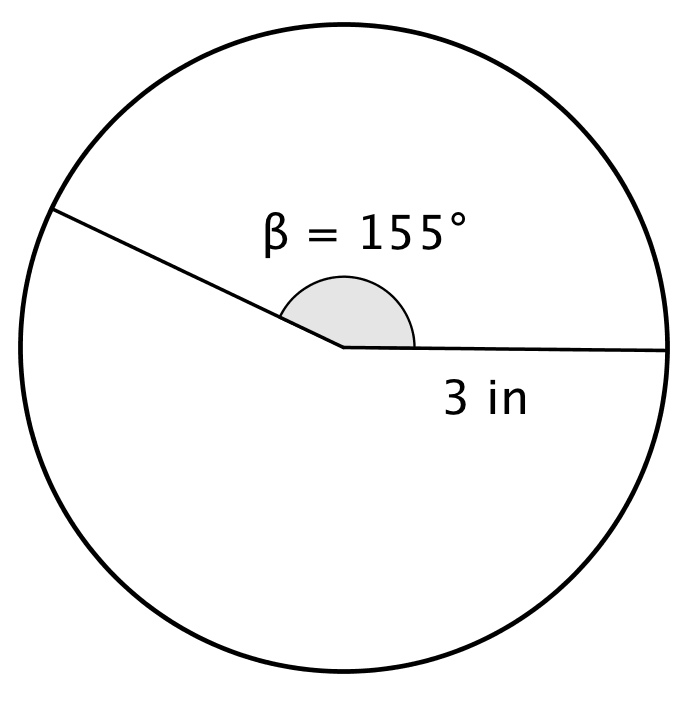
\includegraphics{sector2}}
 \vfill
\item Determine the area of the circular sector with central angle $\beta$ above. 
\end{enumerate}


\vfill









\end{enumerate}

\noindent \textbf{Student Learning Outcomes Check}

\begin{enumerate}
\item Can you find degree and radian measure?
\item Can you determine coterminal angles?
\item Are you able to determine arc length and area of a sector of a circle?
\end{enumerate}

\noindent \textbf{If any of your answers were no, please ask about these topics in class.}

